\chapter[Background on Iterative Decoding]{Background on Iterative
Decoding}\label{iterativeBG}

In this chapter we focus on the LDPC code performance in the low BER
region, and discuss the so-called ``error-floor" phenomenon. We
introduce the combinatorial object termed absorbing set, and relate
it to some existing concepts form the literature. Having defined an
absorbing set, in the next chapter we focus on the detailed
theoretical analysis of absorbing sets for a family of high-rate
array-based LDPC codes.

\section{LDPC Codes, Message Passing Algorithms and Error Floors}

 Empirically,
LDPC codes perform very well when decoded iteratively using
message passing algorithms, despite the fact that such decoding
algorithms are suboptimal on graphs with cycles (and graphs
defining LDPC codes inevitably contain cycles). An added
attractive feature of message passing algorithms is their low
complexity.

However, it is also known \cite{mackay}, \cite{richardson}, that
LDPC codes often exhibit an error floor phenomenon, whereby the bit
error rate (BER) vs. signal to noise ratio (SNR) curve shows a
significant decrease in the slope in the very low BER region. An
example of the error-floor behavior is shown in
Figure~\ref{errorfig} (reproduced from \cite{zhang06}) for the
Reed-Solomon based LDPC code, where different error curves
correspond to specified number of iterations. The error floor
implies that a significant increase in the signal power is needed
for only a marginal improvement in the bit error rate. It is
attributed to the suboptimal nature of the message passing
algorithms on graphs with cycles.

For many applications, including data storage, gigabit ethernet, and
satellite communications, it is imperative to reach this low BER
region without requiring a major increase in SNR. This region,
however, is out of the reach of pure software simulations, and
consequently the limitations of a given LDPC code under
message-passing decoding in the very low BER region are largely
unknown.

In order to explain and analyze the dominant causes of decoding
failures we introduce the notion of an absorbing set in the next
section. The absorbing sets are related to (but not entirely
equivalent to) previously introduced structures, including stopping
sets \cite{di_stop}, trapping sets \cite{richardson}, near codewords
\cite{mackay} and pseudo-codewords \cite{wainwrig}. Fully absorbing
sets are viewed as fixed points of a bit-flipping algorithm (which
itself is a simplest form of message passing and can be viewed as a
1-bit approximation to the finite-precision message passing decoding
algorithms that are used in practice). Our claim is that if there
are fully absorbing sets smaller that the minimum distance of the
code, the decoder is likely to converge to these objects. As a
result, under iterative decoding, the low BER performance will be
dominated by the number and the size of dominant fully absorbing
sets. This is in contrast to the conventional point of view which
considers the number of minimum distance codewords and the minimum
distance itself to be the key performance metric of a code.


\begin{figure}
\center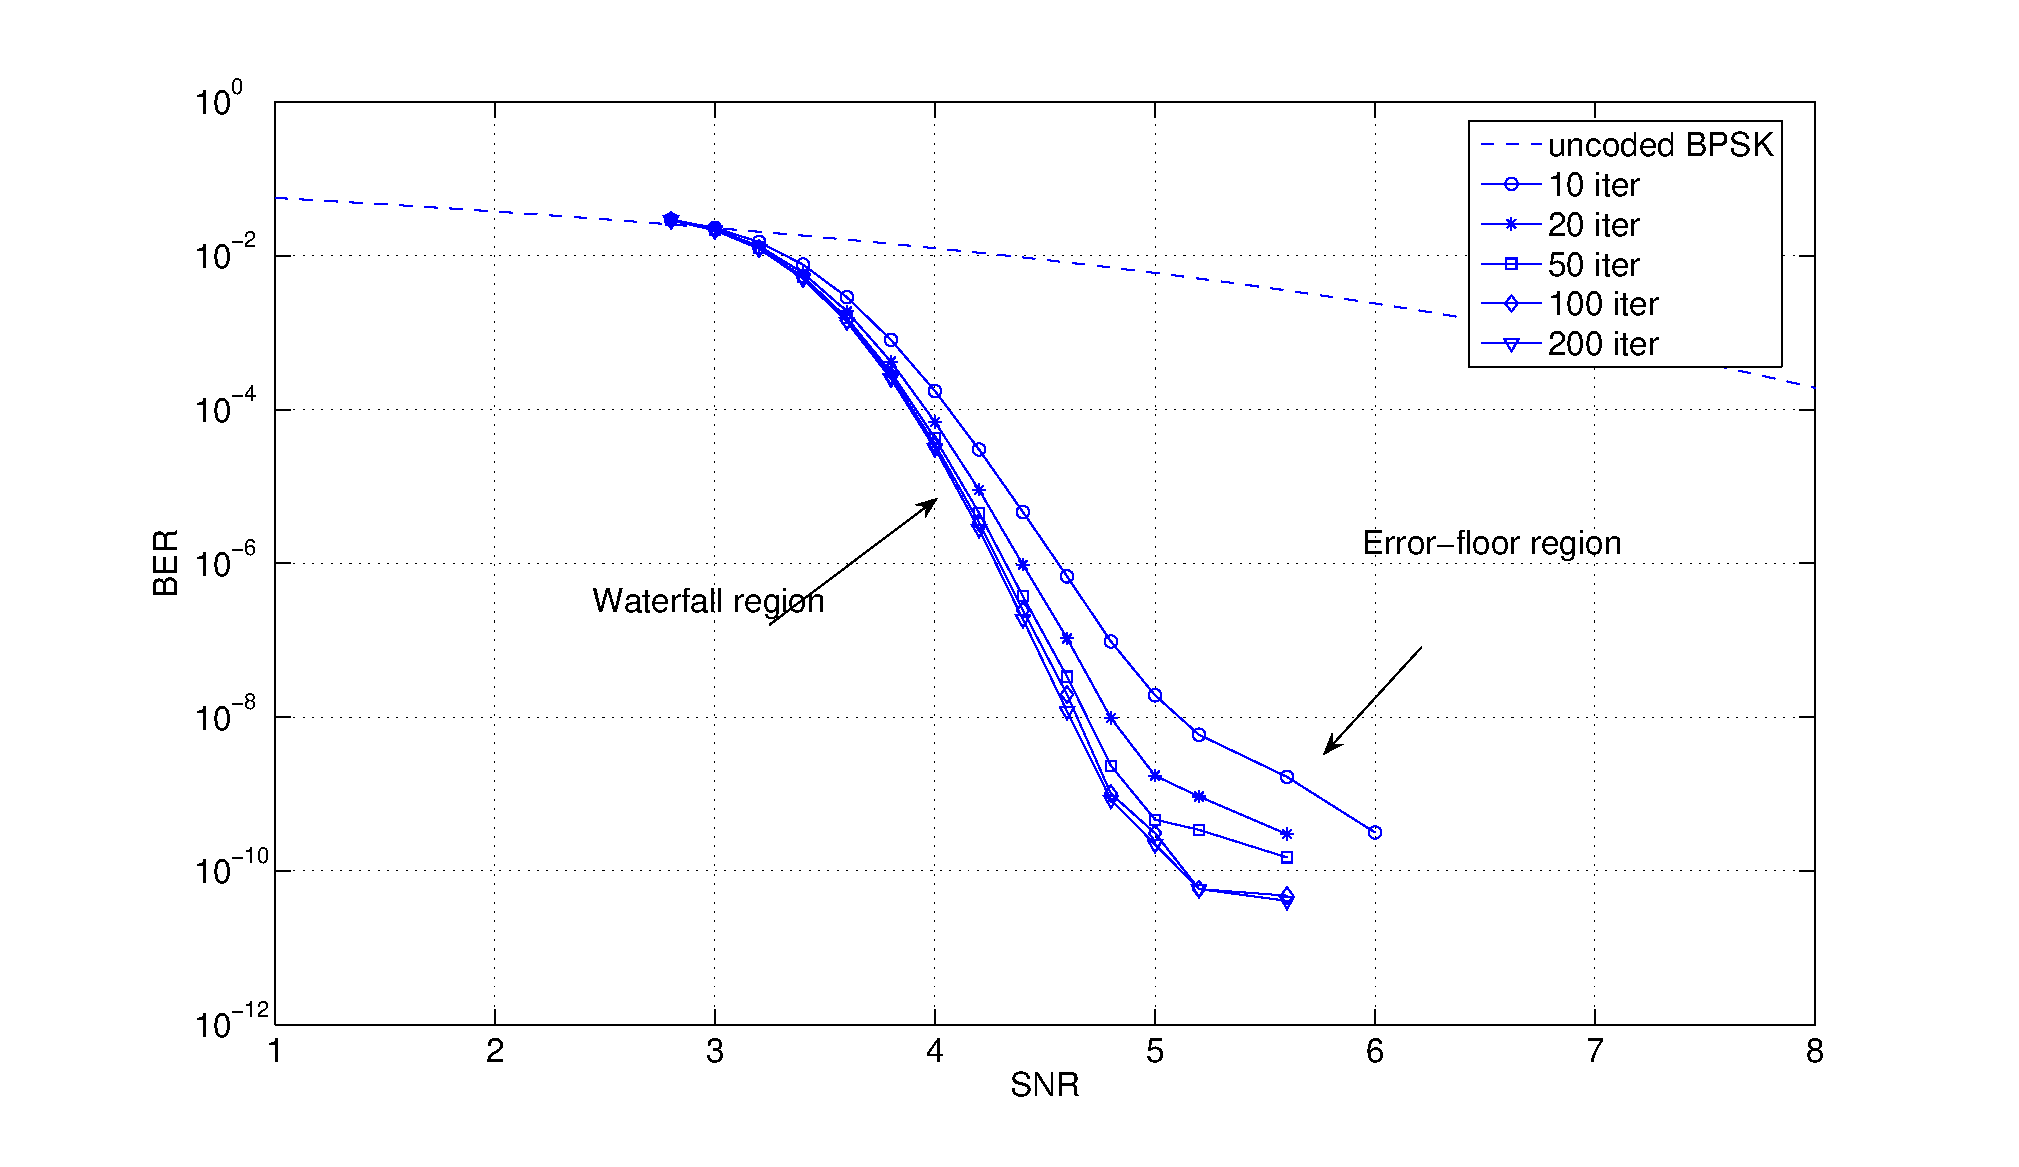
\includegraphics[width=4.75in,keepaspectratio]{iter_globecom3.ps}
\caption{An example of error floor.} \label{errorfig}
\end{figure}


\section{Absorbing sets of LDPC codes}


Several LDPC codes, while having excellent performance for
moderate bit error rate (BER) levels of $10^{-6}$ and above, have
been demonstrated using hardware based emulation \cite{zhang06}
and software clusters \cite{cluster} to suffer from the so-called
``error floor'', see Figure \ref{errorfig}.

This error-floor behavior can be attributed to the suboptimal
nature of the message passing
 algorithms traditionally used in decoding of LDPC codes. Experimental results in
 the low FER region obtained using a hardware emulator
 \cite{zhang06} revealed  that certain structures consisting of short cycles
 organized in particularly detrimental configurations in the Tanner
 graph associated with the parity check matrix of an LDPC code
 cause the decoder to fail by converging to a non-codeword state.


These combinatorial objects that describe the convergence to the
non-codeword state  are called \textit{absorbing sets}. For many
LDPC codes, designed to have sufficiently large minimum distance,
the associated Tanner graphs contain absorbing sets which have
strictly fewer bits than the weight of codewords at the minimum
distance. As a result, the performance of the decoding algorithm
in the low FER region is predominantly dictated by the number and
the structure of minimal absorbing sets, rather than the number of
the minimum distance codewords (which would be the key parameters
in describing the performance of the code under ML decoding).
Before explaining the links between absorbing sets and some
related concepts, including near-codewords and trapping sets, in
Subsection \ref{relcon}, we first provide the formal definition of
these objects.

\subsection{Formal definition}\label{absformal}

Let $G=(V,F,E)$ be a bipartite graph with the vertex set $V \cup
F$, where $V$ and $F$ are disjoint, and with the edge set $E$,
such that there exists an edge $e(i,j) \in E$ iff $i\in V$ and
$j\in F$. One can associate a bipartite graph $G_H=(V,F,E)$ with a
parity check matrix $H$, such that the set $V$ corresponds to the
columns of $H$, the set $F$ corresponds to the rows of $H$, and
$E=\{ e(i,j)| H(j,i)=1\}$. Such a graph $G_H$ is commonly referred
to as the Tanner graph of the parity check matrix $H$ of a code,
\cite{forney}. Elements of $V$ are called ``bit nodes'' and
elements of $F$ are called ``check nodes''. %The Tanner graph
%associated with $H_{p,\gamma}$ does not have any cycles of length
%4, and thus the girth is at least 6 \cite{helles}.
For the subset
$D$ of $V$ we let $N_D$ denote the set of check nodes neighboring
the elements of $D$.

For a subset $D$ of $V$, let $\mathcal{E}(D)$ (resp.
$\mathcal{O}(D)$) be the set of neighboring vertices of $D$ in $F$
in the graph $G$ with even (resp. odd) degree with respect to $D$.
Given an integer pair $(a,b)$, an $(a,b)$ \emph{absorbing set} is
a subset $D$ of $V$ of size $a$, with $\mathcal{O}(D)$ of size $b$
and with the property that each element of $D$ has strictly fewer
neighbors in $\mathcal{O}(D)$ than in $F\backslash
\mathcal{O}(D)$. We say that an $(a,b)$ absorbing set $D$ is an
$(a,b)$ \emph{fully absorbing set}, if in addition, all bit nodes
in $V\backslash D$ have strictly more neighbors in $F\backslash
\mathcal{O}(D)$ than in $\mathcal{O}(D)$.

An example of an $(a,b)$ absorbing set with $a=4$, $b=4$ is given
in Fig. \ref{abs44}, where full circles constitute the set $D$,
full squares constitute the set $\mathcal{O}(D)$, empty squares
constitute the set $\mathcal{E}(D)$, $E(D,\mathcal{O}(D))$ is
given by solid lines, and $E(D,\mathcal{E}(D)$ is given by dashed
lines. Observe that each element in $D$ has more even-degree than
odd-degree neighbors. All check nodes not in the picture are
denoted by empty squares. For this set to be a fully absorbing
set, every bit node not in the figure should also have strictly
more empty squares than full squares as neighbors.



%In the remainder, when we say that the $(a,b)$ absorbing sets do
%(do not) exist for a particular code, we will implicitly refer to
%the existence (non existence) of $(a,b)$ absorbing sets in the
%Tanner graph associated with the given code.

Note that $D \subseteq V$ is a fully absorbing set iff for all $v$,
$wt$$(Hx_{D \Delta v})$ $>$ $wt$$(Hx_D)=b$, where $D \Delta v$
denotes the symmetric difference between $D$ and $\{v\}$, $wt(y)$ is
the Hamming weight of a binary string $y$, and $x_D$ is a binary
string with support $D$.

\begin{figure}
\center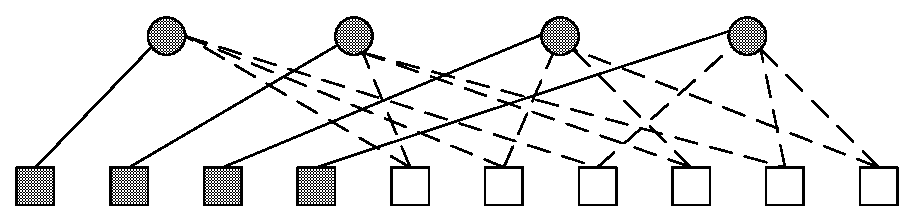
\includegraphics[width=3.0in,height=0.9in]{Drawing11.eps}
\caption{An example of a (4,4) absorbing set} \label{abs44}
\end{figure}


\comment{Moreover, an $(a,b)$ absorbing set can also be
interpreted as follows. For an integer $a$ let $c_a:=c+x_a$, where
$c$ is an arbitrary codeword in the code with the parity check
matrix $H$, and where $x_a$ is a binary vector with non zero
entries in precisely $a$ positions. Let $s_a=Hc_a$, and let $b$ be
the weight of $s_a$. If the weight of $s_a$ strictly increases
when the support of $x_a$ is decreased, the vertex induced
subgraph in $G_H$ induced by the support of $x_a$ and the support
of $s_a$ represents an $(a,b)$ absorbing set.}



We have introduced the notion of absorbing sets to qualitatively
describe the convergent non-codeword state of the message passing
algorithms, when the transmission channel is additive white
gaussian noise (AWGN). In the asymptotic limit given by the bit
flipping algorithm, the configuration described as a fully
absorbing set is stable, since each bit node receives strictly
more messages from the neighboring checks that reinforce its value
than messages that suggest the opposite bit value.

\subsection{Related Work and Existing Concepts}\label{relcon}

The observation that  the low BER/FER performance of finite length
LDPC codes under iterative decoding is guided by non-codewords is
not new. One of the first such attempts to explain these findings
was described in \cite{mackay} where it was recognized that
non-codewords, rather than minimum distance codewords, can attribute
to the error floor. There, the notion of a near-codeword was
introduced. An $(a,b)$ near-codeword refers to a binary string
$\mathbf{s}$ of weight $a$ whose syndrome $\mathbf{s}H^T$ has weight
$b$. A fully absorbing set can be viewed as a near codeword as
defined in \cite{mackay}, though the reverse is not true, since a
near codeword does not necessarily describe a stable configuration.

The trapping sets were introduced in \cite{richardson}  as a part
of the study of error floors of LDPC codes, which pioneered a
simulation-emulation approach. Trapping sets as defined in
\cite{richardson} carry an operational, decoder dependent
definition. In addition, they are defined as a union of all bits
that are not eventually correct, and thus permit a situation in
which the decoder oscillates among a finite number of states.

Stopping sets introduced and studied in detail in \cite{di_stop}
refer to the subgraph of the Tanner graph with the property that
no check node relative to this subgraph has degree 1. These sets
describe stable combinatorial configurations in the context of a
binary erasure channel (BEC), since the decoder halts once it
encounters a stopping set in which all bit nodes were erased. The
stopping sets have been shown to be a very useful tool in
understanding the performance of LDPC codes on erasure channels,
both for finite-length codes \cite{kashyap:03} as well as the
asymptotic behavior of LDPC code ensambles, \cite{orlitsky:05}.
Nevertheless, such analysis cannot be directly applied to an AWGN
channel since the nature of errors is different.

Additional related notions previously introduced in the literature
include pseudo-codewords \cite{wainwrig} and elementary trapping
sets \cite{milenkov}. Note that the pseudo-codewords are defined
in the context of the linear programming based decoding and their
connection with the convergent non-codeword states of the
iterative decoding algorithms though interesting is not yet fully
established. Pseudo-codewords were also studied in \cite{vontobel}
where it was observed that under so-called graph cover decoding,
pseudo-codewords in the covers of the bipartite graph, along with
the actual codewords, compete to be the best estimate produced by
the decoder. Loop calculus method discussed in \cite{chertkov}
provides a way to improve linear programming based decoding once
the so-called critical loop is identified. While for short codes,
as the (155,64) LDPC code discussed in \cite{chertkov}, one loop
may be sufficient to describe a critical state, it would be
interesting to investigate how this concept extends to larger
codes. While \cite{chertkov} uses a search algorithm to find
``bad'' configurations for the (155,64) LDPC code, one could,
based on the structure of the parity check matrix of this code,
analytically describe dominant absorbing sets, and then use these
as a starting point for further analysis. It would be interesting
to further pursue this connection.

Elementary trapping sets are defined as subgraphs in the Tanner
graph in which each check satisfied with respect to this subgraph
has degree 2 and each check  unsatisfied with respect to this
subgraph has degree 1, \cite{milenkov}. \comment{Note that for
example a cycle of length $g$  where $g$ is the girth of the Tanner
graph satisfies the definition of the elementary trapping set.
However, when the bit node degree is large enough, say larger than
4, the message passing
 decoder will not converge to such a configuration since there will
be strictly more unsatisfied than satisfied checks to pull it away
from this configuration.} In a loose sense, one may view absorbing
sets as consisting of a union of elementary trapping sets in some
cases.
